\documentclass[journal,twoside,web]{ieeecolor}
\usepackage{generic}
\usepackage{cite}
\usepackage{amsmath,amssymb,amsfonts}
\usepackage{algorithmic}
\usepackage{graphicx}
\usepackage{algorithm,algorithmic}
\usepackage{hyperref}
\hypersetup{}
\usepackage{textcomp}
\usepackage{array}
\usepackage{subfiles}
\usepackage{float}

\def\BibTeX{{\rm B\kern-.05em{\sc i\kern-.025em b}\kern-.08em
    T\kern-.1667em\lower.7ex\hbox{E}\kern-.125emX}}
\markboth{\journalname, VOL. XX, NO. XX, XXXX 2024}
{Kadambi \MakeLowercase{\textit{et al.}}: Detecting Activities of Daily Living in Egocentric Video}

\begin{document}
\title{Detecting Activities of Daily Living in Egocentric Video to Contextualize Hand Use at Home in Outpatient Neurorehabilitation Settings}
\author{Adesh Kadambi, \IEEEmembership{Member, IEEE} and José Zariffa, \IEEEmembership{Senior Member, IEEE}
    \thanks{This work was supported by the Craig H. Neilsen Foundation (grant number 542675), the Praxis Spinal Cord Institute, the Ontario Early Researcher Award program (ER16–12-013), and the Canadian Institutes of Health Research (grant number 13556838).}
    \thanks{Adesh Kadambi is with the KITE - Toronto Rehabilitation Institute, University Health Network, Toronto, ON, Canada and the Institute of Biomedical Engineering, University of Toronto, Toronto, ON, Canada (e-mail: adesh.kadambi@mail.utoronto.ca).}
    \thanks{José Zariffa is with the KITE - Toronto Rehabilitation Institute, University Health Network, Toronto, ON, Canada, and the Institute of Biomedical Engineering, the Rehabilitation Sciences Institute, Faculty of Medicine, and the Edward S. Rogers Sr. Department of Electrical and Computer Engineering, University of Toronto, Toronto, ON, Canada (e-mail: jose.zariffa@utoronto.ca).}
}

\maketitle

\begin{abstract}
Wearable egocentric cameras and machine learning have the potential to provide clinicians with a more nuanced understanding of patient hand use at home after stroke and spinal cord injury (SCI). However, they require detailed contextual information (i.e., activities and object interactions) to effectively interpret metrics and meaningfully guide therapy planning. We demonstrate that an object-centric approach, focusing on what objects patients interact with rather than how they move, can effectively recognize Activities of Daily Living (ADL) in real-world rehabilitation settings. We evaluated our models on a complex dataset collected in the wild comprising 2261 minutes of egocentric video from 16 participants with impaired hand function. By leveraging pre-trained object detection and hand-object interaction models, our system achieves robust performance across different impairment levels and environments, with our best model achieving a mean weighted F1-score of 0.78 ± 0.12 and maintaining an F1-score over 0.5 for all participants using leave-one-subject-out cross validation. Through qualitative analysis, we observe that this approach generates clinically interpretable information about functional object use while being robust to patient-specific movement variations, making it particularly suitable for rehabilitation contexts with prevalent upper limb impairment.
\end{abstract}

\begin{IEEEkeywords}
activity detection, egocentric video, hand-object interaction, object detection, outpatient neurorehabilitation, spinal cord injury, stroke, wearable technology
\end{IEEEkeywords}

\section{Introduction}
\IEEEPARstart{R}{egaining} hand function for Activities of Daily Living (ADLs) is a top priority for individuals with stroke or spinal cord injury (SCI) during community reintegration \cite{Anderson2004-ck, Purton2023-ad}. While these activities are critical for autonomy and societal integration, current clinical assessment methods rely heavily on direct observation and patient self-reporting. These traditional approaches are limited by recall bias and provide only snapshots of function in clinical settings, failing to capture the diversity of real-world environments and compensatory strategies patients develop at home \cite{Adams1999-ie}. This gap between clinical assessment and actual home function presents a significant challenge in designing targeted rehabilitation interventions.

Wearable egocentric cameras combined with computer vision offer a promising solution for capturing real-world hand function. We previously developed a framework \cite{Bandini2022-rs} that monitors hand use at home by analyzing movement patterns and hand-object interactions, delivering these metrics via a clinical dashboard \cite{Kadambi2023-iv}. However, subsequent evaluation of this system revealed a critical insight into clinical needs: while quantitative metrics were acknowledged, therapists overwhelmingly preferred reviewing video footage to understand patient performance, finding the raw video more valuable than graphical summaries for interpreting functional capabilities and limitations in the home environment \cite{Kadambi2024-fy}. This aligns with established clinical assessment practices like the Graded Redefined Assessment of Strength Sensibility and Prehension (GRASSP) \cite{Kalsi-Ryan2012-pr} or Action Research Arm Test (ARAT) \cite{Yozbatiran2008-ac}, where therapists evaluate functional recovery through a patient's ability to manipulate objects in daily tasks. This preference underscores the need for contextual information, specifically information about ADLs and object interactions being performed, to make quantitative hand-use data meaningful \textit{and} to enable efficient navigation of video data within the dashboard for qualitative assessment \cite{Kadambi2024-fy}. Therefore, providing automated ADL context becomes essential for enhancing the clinical utility of home monitoring systems that rely on quantitative metrics.

Recent approaches in egocentric activity recognition that directly process video sequences, such as 3D Convolutional Neural Networks (CNNs) \cite{Carreira2017-iz, Feichtenhofer2018-ac} and vision transformers \cite{Bertasius2021-re} \cite{Liu2021-tq}, have been driven by the availability of extensive egocentric datasets like EPIC-KITCHENS \cite{Damen2020-ep} and Ego4D \cite{Grauman2021-pg}. However, these approaches do not account for some key challenges in rehabilitation contexts: (1) they typically require extensive training data with consistent movement patterns, which may not be available or appropriate for patients who develop individualized compensatory strategies \cite{Jones2017-zu}, (2) they often operate as black boxes, making their predictions difficult for therapists to interpret and trust, and (3) they are generally constrained to recognizing activities from a predetermined set, limiting their ability to capture the diverse and evolving ways patients accomplish tasks during recovery.

To address these challenges and meet the identified clinical need for activity and object context, we propose an object-centric approach that focuses on what objects patients interact with rather than how they move---a crucial aspect of activity recognition that has been previously validated in literature \cite{Fathi2011-hk, Pirsiavash2012-ly, Nabiei2015-wb, Lonini2016-wg, Granada2020-ge}. This strategy offers three key advantages for rehabilitation settings: (1) flexibility in recognizing activity categories based on object interaction patterns rather than requiring specific predefined activities, (2) interpretable results that align with clinical assessment methods by providing clear information about functional object use, and (3) feasible deployment by leveraging existing, pre-trained object detection and interaction models without requiring patient-specific training data.

The primary contribution of our work is demonstrating that applying a simplified object-based approach can achieve robust activity recognition in real-world home settings across different impairment levels, specifically to provide the functional context required by therapists. This functional context supplements information about quantity \cite{Bandini2022-rs} and quality \cite{Dousty2023-kn, Zhao2024-bc} of hand use in existing frameworks \cite{Kadambi2023-iv}. This work bridges the gap between automated monitoring and clinical utility, providing therapists with the contextual information they need for rehabilitation planning.

\section{Methods}
\subsection{Dataset \& Preprocessing}

We performed a retrospective analysis of the dataset previously described by Bandini \textit{et al}. \cite{Bandini2022-rs}, where 21 participants recorded themselves performing an array of real ADLs within their home environments without any imposed constraints, following the recording protocol outlined by Tsai \textit{et al}. \cite{Tsai2020-up}.

The recordings were segmented into one-minute snippets. Video snippets were excluded from analysis if they met any of the following criteria: (1) contained sensitive or identifying information (e.g., toileting activities, faces, passwords, bank statements, etc.), (2) insufficient visibility (e.g., extremely low lighting conditions / black screen), or (3) no discernible hand or object movement (e.g., static scenes where the participant was stationary). These exclusion criteria were established to ensure data quality and reliable model performance, as segments without visible objects or interactions provide no informative features for our object-centric approach. The final dataset, after exclusions, is comprised of 2261 one minute egocentric video snippets obtained from 16 participants with impaired hand functionality (American Spinal Injury Association Impairment Scale A-D; Level of Injury C3-C7) due to SCI. The number of video snippets varied per participant, ranging from a minimum of 7 minutes to a maximum of 229 minutes, with an average duration of 141.31 ± 72.91 minutes.

Video snippets were manually classified into seven predefined ADL categories, aligning with the American Occupational Therapy Association's Occupational Therapy Practice Framework \cite{Aota2020-xa} and chosen based on the most common activities observed in the dataset. The categories included: \textbf{Self-Feeding} (257 instances), involving tasks related to setting up and consuming meals, such as manipulating utensils and bringing food/drink to the mouth; \textbf{Functional Mobility} (207 instances), encompassing movements like wheelchair use and transfers, focusing on interactions with mobility aids and the environment; \textbf{Grooming \& Health Management} (172 instances), covering personal care routines like hygiene, medication management, and exercise; \textbf{Communication Management} (428 instances), involving the use of devices like phones or computers; \textbf{Home Management} (407 instances), relating to tasks for maintaining personal and household environments, such as cleaning or organizing; \textbf{Meal Preparation and Cleanup} (625 instances), encompassing planning, preparing, serving meals, and subsequent cleanup using kitchen tools and appliances; and \textbf{Leisure \& Other Activities} (165 instances), representing non-obligatory activities during discretionary time involving object manipulation. In cases where multiple ADLs were observed in a single snippet, the snippet was assigned the label of the predominant ADL (i.e., the one performed for the longest duration within the minute).

\subsection{Feature Engineering Pipeline}

Our feature engineering pipeline (Fig. \ref{fig:pipeline}) consists of three main stages: object detection, interaction detection, and feature generation.

\begin{figure*}[t!]
    \centering
    \includegraphics[width=1\linewidth]{figs/flowchart.png}
    \caption{Pipeline for detecting ADLs from egocentric videos. Steps in red indicate operations on the entire 1-minute video snippet while steps in green indicate operations on individual frames.}
    \label{fig:pipeline}
\end{figure*}

\subsubsection{Object Detection}

For object detection, we employed the pre-trained Detic model \cite{Zhou2022-fl}, which detects a broad range of objects in each video frame. The detected objects were mapped to 29 functional categories relevant to rehabilitation (e.g., "kitchen utensils", "electronics", "wheelchair/walker") through a predefined mapping scheme to standardize object classifications.

\subsubsection{Interaction Detection}

To identify object interactions, we utilized the pre-trained 100DOH hand-object interaction model \cite{Shan2020-gh}. Objects were classified as active or passive based on their spatial relationship with detected hand interactions. Specifically, an object was considered active if a Detic bounding box had an intersection over union greater than 0.8 with a 100DOH object bounding box. This distinction is clinically relevant as it differentiates between objects that patients can effectively manipulate and those that appear passively in the scene.

\subsubsection{Expected Model Performance}

Both Detic \cite{Zhou2022-fl} and 100DOH \cite{Shan2020-gh} were evaluated on our dataset to assess their suitability for generating object-based features. Using a stratified sampling approach, we randomly selected two videos per participant for each ADL category, resulting in a subset of 1,482 images with 4,757 manually annotated bounding boxes, representing approximately 5\% of the total dataset \cite{Kadambi2023-hx}. For object detection, Detic achieved a micro-average mean average precision (mAP) of 0.37 for all objects (active and passive) and 0.63 for active objects only. These values reflect our ground truth labeling strategy, where we annotated only objects directly relevant to the ADLs, rather than all objects present in the scene. As a result, many objects correctly detected by Detic—such as background items not tied to the activity—were excluded from our ground truth and thus classified as false positives in the mAP calculation. This does not indicate poor model performance, but rather highlights the selective focus of our annotations on functionally significant objects. To complement this, we also report micro-average mean average recall (mAR) of 0.56 for all objects and 0.71 for active objects, emphasizing the model's ability to detect the ground truth objects we prioritized. For interaction detection, the 100DOH model \cite{Shan2020-gh} was evaluated on 632,180 manually annotated frames from 13 participants, achieving a median F1-score of 0.80 (0.67-0.85), confirming its strong performance on our dataset \cite{Bandini2022-rs}.

\subsubsection{Feature Generation}

For each one-minute video segment, frames were extracted at 1 FPS. From these frames, we generated two types of feature vectors, or Bags of Objects (BoO): (1) Binary presence vectors, which record whether each object category appears at least once per frame (e.g., 1 if tableware is present, 0 if not) and sum these occurrences across all frames in each 1-minute segment; and (2) Counts vectors, which tally the total number of instances of each object category detected per frame (e.g., 3 tableware if three items are detected) and sum these counts across all frames in the segment.

Both representations underwent row-wise min-max scaling to normalize features within each segment, emphasizing the relative presence of objects rather than absolute counts. This normalization strategy makes our approach more robust to variations in recording duration and activity speed across participants with different impairment levels.

\subsection{ADL Classification}

We evaluated a range of classification models to assess different learning approaches on our object-based features. Models included logistic regression (LR), chosen for its interpretability and suitability as a linear baseline; random forest (RF), gradient boosting (GB), and XGBoost (XGB), selected for their ability to capture non-linear relationships and robustness; and a multi-layer perceptron (MLP), included as a standard neural network baseline.

The classification models were implemented using scikit-learn. To mitigate the class imbalance observed across ADL categories, we employed balanced class weights within the LR and RF models. The MLP utilized adaptive learning rates and early stopping based on validation loss to prevent overfitting. For GB and XGB, we used the default hyperparameters provided by scikit-learn and the XGBoost library, respectively. This decision was made to maintain simplicity and reduce the risk of overfitting through extensive tuning, given the size and variability of our dataset.

\subsection{Evaluation Framework}

To assess the generalization capability of our models to new, unseen participants, we employed leave-one-subject-out cross-validation (LOSO CV) \cite{Gholamiangonabadi2020-dd}. This evaluation strategy is particularly relevant in rehabilitation contexts, where inter-individual variability in movement patterns and compensatory strategies due to impairment can significantly impact model performance.

Model performance was primarily evaluated using the weighted F1-score, which accounts for class imbalance by weighting the F1-score of each class by its support (the number of true instances for that class). We also report the percentage of participants for whom the model achieved a weighted F1-score greater than 0.5, providing insight into the model's consistency across individuals—a crucial factor for clinical utility, as a monitoring system must be reliable for different patients.

We conducted an ablation study comparing different feature engineering choices (binary presence vs. counts vs. both, with and without the active object distinction) to identify the most effective feature representation for this task. Classification models trained without the active object distinction used BoO vectors generated solely from the Detic \cite{Zhou2022-fl} object detections, prior to applying the 100DOH \cite{Shan2020-gh} interaction model. This analysis helps elucidate the contribution of different feature components to ADL recognition performance in this specific patient population.


\section{Results}
The impact of including active object information was consistent across different feature representations (Table \ref{tab:ablation}). Using logistic regression, our best performing classifier, as an example, we observe the weighted F1-score improved from 0.70 ± 0.14 to 0.73 ± 0.13 with the inclusion of active objects when using counts, from 0.73 ± 0.15 to 0.78 ± 0.12 when using binary presence, and from 0.72 ± 0.13 to 0.77 ± 0.13 when using both.

\begin{table}[h]
    \centering
    \caption{Performance of classifiers across configuration settings.}
    \renewcommand{\arraystretch}{1.5}
    \setlength{\tabcolsep}{3pt}
    \begin{tabular}{
    |>{\centering\arraybackslash}m{0.2\linewidth}
    |>{\centering\arraybackslash}m{0.12\linewidth}
    |>{\arraybackslash}m{0.25\linewidth}
    |>{\arraybackslash}m{0.2\linewidth}|
    }
    \hline
        \textbf{Configuration}
        &
        \textbf{Active Objects}
        &
        \textbf{Mean Weighted \newline F1-score}
        % \textbf{Mean F1-score}
        &
        \textbf{Percentage of \newline Participants $>$0.5 F1-score}
        % \textbf{Pct over 0.5}
        % &
        % \textbf{OvR Weighted ROC AUC}
        \\
    \hline
    % COUNTS
        Counts
        &
        &
        GB: $0.66 \pm 0.23$ \newline
        LR: $0.70 \pm 0.14$ \newline
        MLP: $0.65 \pm 0.20$ \newline
        RF: $0.65 \pm 0.22$ \newline
        XGB: $0.67 \pm 0.22$
        &
        GB: 81\% \newline
        LR: 88\% \newline
        MLP: 81\% \newline
        RF: 75\% \newline
        XGB: 81\%
        % &
        % GB: 0.91 \newline
        % LR: 0.90 \newline
        % MLP: 0.88 \newline
        % RF: 0.91 \newline
        % XGB: 0.91
        \\
    \hline
    % COUNTS + ACTIVE
        Counts
        & \checkmark
        &
        GB: $0.69 \pm 0.20$ \newline
        LR: $0.73 \pm 0.13$ \newline
        MLP: $0.70 \pm 0.18$ \newline
        RF: $0.72 \pm 0.22$ \newline
        XGB: $0.70 \pm 0.20$
        &
        GB: 88\% \newline
        LR: 94\% \newline
        MLP: 81\% \newline
        RF: 81\% \newline
        XGB: 88\%
        % &
        % GB: 0.92 \newline
        % LR: 0.91 \newline
        % MLP: 0.91 \newline
        % RF: 0.92 \newline
        % XGB: 0.92
        \\
    \hline
    % BINARY
        Binary
        &
        &
        GB: $0.70 \pm 0.18$ \newline
        LR: $0.73 \pm 0.15$ \newline
        MLP: $0.65 \pm 0.24$ \newline
        RF: $0.64 \pm 0.24$ \newline
        XGB: $0.69 \pm 0.18$
        &
        GB: 81\% \newline
        LR: 94\% \newline
        MLP: 81\% \newline
        RF: 81\% \newline
        XGB: 88\%
        % &
        % GB: 0.91 \newline
        % LR: 0.93 \newline
        % MLP: 0.91 \newline
        % RF: 0.91 \newline
        % XGB: 0.91
        \\
    \hline
    % BINARY + ACTIVE
        Binary
        & \checkmark
        &
        GB: $0.73 \pm 0.18$ \newline
        \textbf{LR: 0.78 $\pm$ 0.12} \newline
        MLP: $0.73 \pm 0.22$ \newline
        RF: $0.69 \pm 0.25$ \newline
        XGB: $0.74 \pm 0.17$
        &
        GB: 88\% \newline
        \textbf{LR: 100\%} \newline
        MLP: 81\% \newline
        RF: 81\% \newline
        XGB: 88\%
        % &
        % GB: 0.92 \newline
        % \textbf{LR: 0.94} \newline
        % \textbf{MLP: 0.94} \newline
        % RF: 0.92 \newline
        % XGB: 0.93
        \\
    \hline
    % COUNTS + BINARY
        Counts + Binary
        &
        &
        GB: $0.69 \pm 0.20$ \newline
        LR: $0.72 \pm 0.13$ \newline
        MLP: $0.68 \pm 0.18$ \newline
        RF: $0.69 \pm 0.23$ \newline
        XGB: $0.68 \pm 0.17$
        &
        GB: 81\% \newline
        LR: 94\% \newline
        MLP: 88\% \newline
        RF: 81\% \newline
        XGB: 81\%
        % &
        % GB: 0.91 \newline
        % LR: 0.91 \newline
        % MLP: 0.90 \newline
        % RF: 0.90 \newline
        % XGB: 0.91
        \\
    \hline
    % COUNTS + BINARY + ACTIVE
        Counts + Binary
        & \checkmark
        &
        GB: $0.71 \pm 0.19$ \newline
        LR: $0.77 \pm 0.13$ \newline
        MLP: $0.72 \pm 0.16$ \newline
        RF: $0.69 \pm 0.23$ \newline
        XGB: $0.70 \pm 0.17$
        &
        GB: 81\% \newline
        LR: 94\% \newline
        MLP: 94\% \newline
        RF: 81\% \newline
        XGB: 88\%
        % &
        % GB: 0.93 \newline
        % LR: 0.92 \newline
        % MLP: 0.91 \newline
        % RF: 0.92 \newline
        % XGB: 0.93
        \\
    \hline
    \end{tabular}
    \label{tab:ablation}
\end{table}

We observed that binary presence features generally outperformed object counts across all classifiers. This suggests that for ADL classification in rehabilitation settings, the simple presence or absence of objects is more informative than their frequency. Most notably, the combination of binary presence features \textit{with} active object distinction achieved our highest performance (F1: 0.78 ± 0.12) while maintaining F1-scores above 0.5 for all participants. This suggests that distinguishing between objects that patients can actively manipulate versus those that are merely present in their environment provides valuable information for ADL classification. This result also indicates the robustness of our method on data from new participants unseen during training.

Looking at the confusion matrix (Fig. \ref{fig:cm}) from our best performing model, we observe strong performance on ADLs with distinctive object patterns. "Communication Management" shows good diagonal accuracy (0.68), with most misclassifications occurring with "Leisure \& Other Activities", likely due to shared electronic device usage patterns. Similarly, "Meal Preparation and Cleanup" and "Self Feeding" show strong diagonal values (0.84 and 0.78 respectively), characterized by distinctive kitchen objects and tableware. However, the model showed lower performance on "Grooming \& Health Management" and "Leisure \& Other Activities", which had the fewest training samples (172 and 165 instances respectively) and more variable object patterns.

\begin{figure}[h]
    \centering
    \includegraphics[width=1\linewidth]{figs/LR-confusion-matrix-10x8.png}
    \caption{Confusion matrix for Logistic Regression using binary presence bag-of-objects and including flags for active objects. CM - Communication Management; FM - Functional Mobility; GHM - Grooming \& Health Management; HM - Home Management; LO - Leisure \& Other Activities; MPC - Meal Preparation and Cleanup; SF - Self-Feeding.}
    \label{fig:cm}
\end{figure}

We evaluated our approach's robustness to imperfect object detection by comparing performance on a subset of data (approximately 5\% of our dataset) where we had manual ground truth object annotations (Table \ref{tab:ground-truth}). Despite only modest object detection performance on our dataset, the ADL classification performance remained stable whether using automatically detected objects (F1: 0.65 ± 0.16) or ground truth annotations (F1: 0.62 ± 0.17). This suggests that our activity recognition approach is robust to object detection errors, as even imperfect object detection provides sufficient information for reliable ADL classification.

\begin{table}[h]
    \centering
    \caption{Performance of LR trained using the binary presence feature vector with active objects on ground truth bounding boxes versus detected objects on a subset (\~5\%) of the data.}
    \renewcommand{\arraystretch}{1.5}
    \setlength{\tabcolsep}{3pt}
    \begin{tabular}{
    |>{\centering\arraybackslash}m{0.25\linewidth}
    |>{\centering\arraybackslash}m{0.25\linewidth}
    |>{\centering\arraybackslash}m{0.25\linewidth}|
    }
    \hline
        \textbf{Training Data}
        &
        \textbf{Mean Weighted \newline F1-score}
        &
        \textbf{Percentage of \newline Participants $>$0.5 F1-score}
        \\
    \hline
        Ground Truth
        &
        $0.62 \pm 0.17$
        &
        69\%
        \\
    \hline
        Detected Objects
        &
        $0.65 \pm 0.16$
        &
        75\%
        \\
    \hline
    \end{tabular}
    \label{tab:ground-truth}
\end{table}

Qualitative analysis reveals cases where predicted labels, while technically incorrect, may be clinically interpretable. For example, in Fig. \ref{fig:qual} (Left), the participant is taking medication in the kitchen with drinkware present. While ground truth labels this as "Grooming \& Health Management", the model's prediction of "Self Feeding" reflects the similar object patterns between medication consumption and eating activities. Such cases highlight the overlap in object usage patterns across different ADLs and suggest potential refinements in how activities are categorized for rehabilitation assessment.

\begin{figure*}[t!]
    \centering
    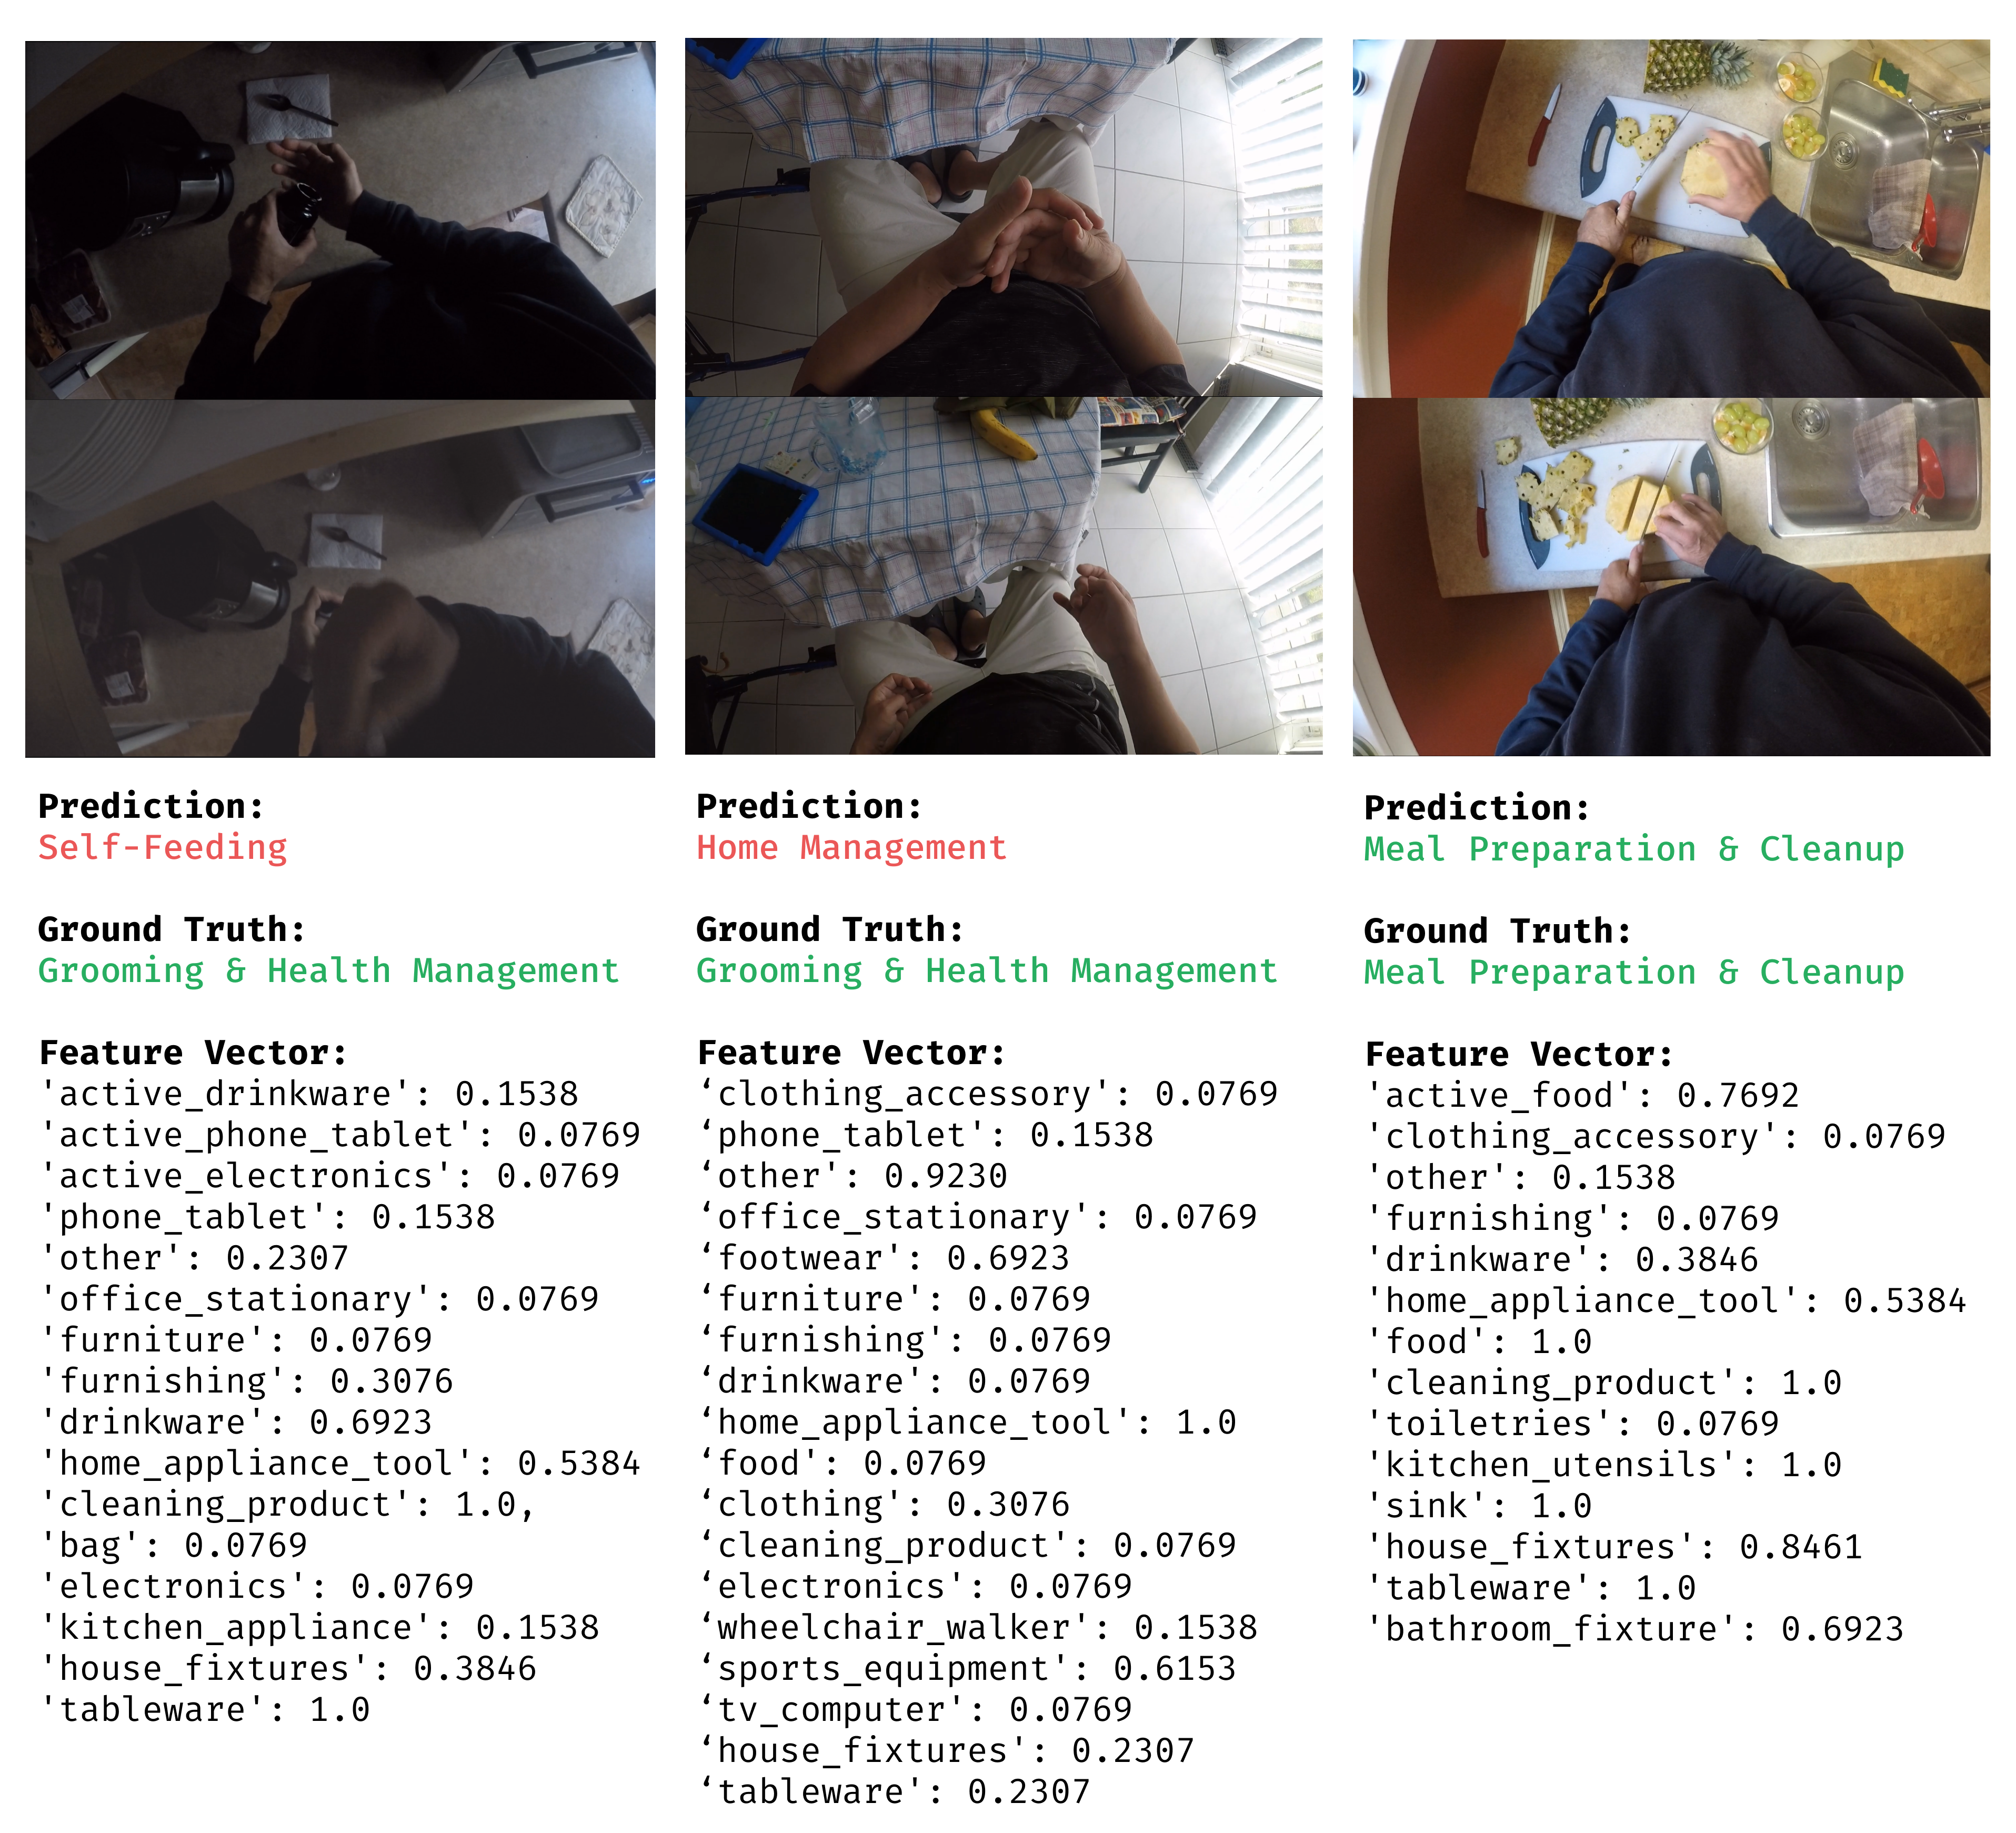
\includegraphics[width=1\linewidth]{figs/qual-frames.png}
    \caption{Qualitative evaluation of ADL calssification displaying sample frames from the video snippets, followed by the ADL prediction, ADL ground truth, and the min-max normalization of detected objects from our best performing model, LR with active objects and binary presence.}
    \label{fig:qual}
\end{figure*}

\section{Discussion}
Understanding how patients use their hands in functional tasks at home is crucial for effective rehabilitation planning. While detailed analysis of movement patterns and quality remains essential, contextualizing these movements within daily activities provides therapists with crucial insights for treatment planning. Our work demonstrates that automated ADL recognition can provide this contextual layer, complementing existing approaches to movement analysis in rehabilitation settings.

Building on earlier work showing the importance of objects in activity recognition \cite{Surie2007-rr, Wu2007-jc, Palmes2010-lg, Escorcia2022-sj}, we explored an object-centric approach to address the specific clinical need for activity context, identified through feedback on our prior work \cite{Kadambi2024-fy}. While traditional approaches like CNNs \cite{Douache2023-ez}, transformers \cite{Li2020-zg, Bertasius2021-re, Liu2021-tq, Pan2023-zq}, multimodal methods \cite{Papadakis2024-ja, Hao2024-ta}, or domain adaptation techniques \cite{Liu2023-sa} excel at fine-grained action recognition (e.g., "cutting tomato"), our objective is different. We aim to provide broader ADL categories (e.g., "Meal Preparation") that help therapists interpret quantitative hand movement metrics within a clinical dashboard \cite{Kadambi2023-iv}. Knowing the ADL and object context allows therapists to normalize expectations for interaction rates and identify relevant video segments efficiently. Our contribution lies not in inventing object-centric recognition, but in demonstrating its practical application using pre-trained models to generate this clinically relevant context. Our object-centric approach aligns with this clinical need by identifying patterns of functional object use within ADL categories, providing interpretable information that complements quantitative metrics as opposed to CNNs and transformers which operate as black boxes.

Our findings reveal that binary presence features consistently outperform object counts, suggesting that for ADL classification in rehabilitation contexts, the ability to interact with specific objects is more informative than interaction frequency. This may be due to inaccuracies in object detections, which may have added additional noise to the model trained on object counts, causing them to overfit to the counts of particular objects. As a result, models trained using binary presence may be robust to inaccurate object detections at the frame-level since the correct objects are detected at some point in the frames of a video snippet.

The addition of active object detection significantly improved classification performance, achieving a mean weighted F1-score of 0.78 ± 0.12 with 100\% of participants maintaining scores above 0.5 with our best model. This robustness across participants is particularly important in rehabilitation, where individual variations in movement patterns and compensatory strategies can significantly impact activity recognition. The stability of our approach even with imperfect object detection suggests its viability for real-world deployment where perfect object recognition cannot be guaranteed.

However, several limitations warrant discussion. First, while our current analysis excluded unsuitable video segments, a deployed system requires automated quality control to handle poor visibility or lack of activity. Future work should integrate mechanisms like low-light enhancement \cite{Singh2019-nd, Peng2022-lc} or motion detection \cite{Shruthi2017-ie} to automatically flag segments unsuitable for analysis, ensuring clinicians receive reliable information from meaningful activities.

Second, the dataset exhibits class imbalance and variability inherent to "in the wild" data collection. Specifically, ADLs like “Grooming \& Health Management” (172 instances) and “Leisure \& Other Activities” (165 instances) had significantly fewer samples compared to categories like “Meal Preparation and Cleanup” (625 instances). This underrepresentation, combined with the inherent diversity of activities within these categories, likely contributed to the lower classification performance observed for these ADLs. Furthermore, variable filming conditions, such as inconsistent lighting or image blur due to movement, common in home environments, also impact object detection performance and pose challenges for classification. While these factors reflect the reality of home monitoring, future work could benefit from targeted data collection to augment underrepresented ADLs or exploring techniques robust to visual variability.

Third, regarding the underlying object detection, while our approach demonstrates robustness, performance could potentially be improved by fine-tuning detection models. Although leveraging large annotated datasets like EPIC-KITCHENS \cite{Damen2020-ep} could enhance detection accuracy for specific action-object interactions, our current use of off-the-shelf pre-trained models (Detic, 100DOH) prioritizes generalizability and deployment feasibility across diverse home environments and impairment levels without requiring extensive, task-specific retraining, which is often impractical in clinical research settings. Future work could explore fine-tuning on relevant public datasets as a potential avenue to boost detection performance, balancing accuracy gains with practical constraints.

Our qualitative analysis identified misclassifications where activities share similar object profiles but differ in intent or sequence, such as mistaking “Self-Feeding” for “Grooming \& Health Management” when medication was taken at a kitchen table (Fig. \ref{fig:qual}, Left). Our current static features capture \textit{which} objects are present and active but lack temporal dynamics. This was an intentional design choice: aiming for flexibility to categorize functional activities based on object context rather than relying on specific movement sequences, which can be highly variable and inconsistent in individuals with neurological impairments using compensatory strategies. While this object-centric focus provides robustness and interpretability, it means our current model, even with active object detection, is insufficient to fully disambiguate activities solely based on overlapping object patterns. The underperformance of counts-based features compared to binary presence (Table \ref{tab:ablation}) further suggests that simple frequency information does not adequately capture the necessary temporal distinctions.

Our simplified strategy for ADL recognition---using only binary object presence and active object detection---can effectively provide the activity context needed by clinicians to interpret hand function metrics. This has practical implications for deployment in rehabilitation settings, as the direct mapping between objects and activities makes the system's decisions transparent and interpretable, crucial for contextualizing hand use metrics in our clinical dashboard \cite{Kadambi2023-iv}. Future work should continue to investigate methods that enhance ADL classification accuracy, particularly for ambiguous cases, while balancing performance with the practical requirements of interpretability and robustness for clinical application. Furthermore, emerging vision-language models (VLMs) or multimodal large language models (LLMs) represent a promising avenue for future exploration. These models could potentially offer richer semantic understanding of video content, generate more descriptive tags automatically, or even enable natural language querying (e.g., "find videos where the patient struggled with cooking"), potentially offering complementary or enhanced ways to retrieve and analyze clinically relevant video segments. Investigating how these advanced models can be effectively and reliably applied within the specific constraints and needs of neurorehabilitation remains an important direction.



\section{Conclusion}
This study demonstrates the feasibility of using an object-centric approach to automatically recognize ADLs from egocentric video in outpatient neurorehabilitation settings. Addressing the clinically identified need for contextual information to interpret quantitative hand-use metrics \cite{Kadambi2024-fy}, our method leverages pre-trained object detection and hand-object interaction models to classify broad ADL categories based on object interaction patterns. Evaluated on a challenging dataset collected "in the wild" from 16 participants with upper limb impairment due to SCI, our approach proved effective and robust.

Our findings indicate that binary presence features, capturing whether specific object categories are interacted with, outperform simple object counts. Furthermore, distinguishing active objects (those being manipulated) significantly enhances classification accuracy. Our best performing model, a logistic regression using binary presence and active object features, achieved a mean weighted F1-score of 0.78 ± 0.12 using LOSO CV, with consistent performance (F1 > 0.5) across all participants.

The primary advantage of this object-centric strategy lies in its interpretability and robustness within the rehabilitation context. By focusing on functional object use rather than specific movement patterns, the approach accommodates the compensatory strategies common in individuals with impairments. It provides clinicians with transparent, understandable information about patient engagement in different ADL categories, directly supporting the interpretation of hand function data presented in clinical dashboards \cite{Kadambi2023-iv}.

While challenges remain, particularly regarding automated video quality control and classifying activities with highly variable object patterns or limited data, our work confirms that object interaction analysis is a viable method for providing essential ADL context. This approach bridges a critical gap by enriching quantitative hand-use data with meaningful functional information, ultimately paving the way for more personalized and effective rehabilitation strategies informed by patients' real-world activities at home.

\appendices
% \section*{Acknowledgment}
\bibliographystyle{IEEEtran}
\bibliography{refs}

\end{document}
